% !Mode:: "TeX:UTF-8"
%!TEX program = xelatex

%\documentclass[bwprint,fontset=windows]{gmcmthesis}
\documentclass[bwprint]{gmcmthesis}

\hypersetup{hidelinks}
\usepackage{subfig}
\usepackage{siunitx}
\usepackage{amsmath,amssymb}
\usepackage{booktabs}
\usepackage{graphicx}
\usepackage{tabularx}
\usepackage{array}
\usepackage{multirow}
\usepackage{caption}
\captionsetup[figure]{justification=centering,font=small,labelsep=quad}
\captionsetup[table]{justification=centering,font=small,labelsep=quad}

% 算法
\usepackage[noend]{algpseudocode}
\usepackage{algorithmicx,algorithm}
\floatname{algorithm}{算法}
\renewcommand{\algorithmicrequire}{\textbf{输入:}}
\renewcommand{\algorithmicensure}{\textbf{输出:}}

% 章节编号
\renewcommand\thesection{\chinese{section}、}
\renewcommand\thesubsection{\arabic{section}.\arabic{subsection}}
\renewcommand\thesubsubsection{\thesubsection.\arabic{subsubsection}}

% 统一表格格式：三线表、表内文字全部居中、紧凑但不拥挤
\newcolumntype{Y}{>{\centering\arraybackslash}X}
\newcolumntype{L}{>{\raggedright\arraybackslash}X}
\newcolumntype{C}[1]{>{\centering\arraybackslash}m{#1}}
\newcolumntype{P}[1]{>{\raggedright\arraybackslash}m{#1}}
\newcommand{\TableSetup}{%
    \centering
    \small
    \setlength{\tabcolsep}{5pt}%
    \renewcommand{\arraystretch}{1.13}%
}
\newcommand{\CompactTableSetup}{%
    \centering
    \footnotesize
    \setlength{\tabcolsep}{4pt}%
    \renewcommand{\arraystretch}{1.08}%
}
\newcommand{\TableNote}[2][0.96\textwidth]{%
    \vspace{0.25em}\par
    \begin{minipage}{#1}
    \small\raggedright #2
    \end{minipage}
}

%===================== 建模论文题目 ======================
\title{全国研究生数学建模竞赛论文标题}
\baominghao{\hspace{6em} 20250900001}
\schoolname{\hspace{5.8em} 中南大学}
\membera{\hspace{6em} 彭铸}
\memberb{\hspace{6em} 郑徐瀚宇}
\memberc{\hspace{6em} 阳挺}
%=======================================================

\begin{document}

\maketitle

\begin{abstract}
% TODO: 摘要
\end{abstract}

\pagestyle{plain}
\maketoc
\clearpage

% =====================================================
% 一、问题重述
% =====================================================
\section{问题重述}

\subsection{问题背景}
% TODO

\subsection{问题重述}
% TODO

\subsection{总体技术路线}
% TODO

% =====================================================
% 二、基本假设与符号说明
% =====================================================
\section{基本假设与符号说明}

\subsection{基本假设}
\begin{enumerate}
    \item % TODO
\end{enumerate}

\subsection{符号说明}
\begin{table}[htbp]
    \TableSetup
    \caption{主要符号说明}
    \renewcommand{\tabularxcolumn}[1]{m{#1}}
    \begin{tabularx}{0.94\textwidth}{@{}C{2.9cm}Y@{}}
        \toprule
        符号 & 含义 \\
        \midrule
        $x_{ij}$ & 样本 $i$ 在第 $j$ 项质量信号上的原始取值 \\
        $s_{ij}$ & 指标方向统一后的质量表示，$s_{ij}\in[0,1]$ \\
        $F_j^{\mathrm{bal}}$ & 第 $j$ 项信号的域均衡经验分布 \\
        $\mathcal{P},\mathcal{N},\mathcal{M}$ & 正向、负向与中心适宜指标集合 \\
        $G_k$、$a_{jk}$ & 第 $k$ 个信息簇及其簇内指标权重 \\
        $K$ & 信息簇个数，取 $K=9$ \\
        $\eta_j$ & 第 $j$ 项信号的领域间方差占比 \\
        $Q_i^{(0)}$ & 样本 $i$ 的初始质量分数 \\
        $r_{ij}$、$I_{ij}$ & 标准化异常度与冲突指示变量 \\
        $C_i$ & 样本 $i$ 的冲突度 \\
        $R_{ij}$、$U_i$ & 证据可靠度与信息簇平均可靠度 \\
        $Q_i^{*}$ & 冲突校正后的质量分数 \\
        $p_i$ & 第 $i$ 个训练域在配方中的份额 \\
        $z_{mk}$、$\phi(\mathbf{p})$ & 标准化验证损失与总体配比表现 \\
        $S_{i\leftarrow j}$ & 份额由领域 $j$ 转向领域 $i$ 的边际替换效应 \\
        $C_{ij}^{\mathrm{mix}}$ & 领域 $i$ 与 $j$ 的互补指数 \\
        $\rho_s$ & Spearman 等级相关系数 \\
        \bottomrule
    \end{tabularx}
\end{table}

% =====================================================
% 三、数据说明与预处理
% =====================================================
\section{数据说明与预处理}

\subsection{数据来源及可信度分层}
% TODO

\subsection{数据口径统一}
% TODO

\subsection{训练、检验及外推数据划分}
% TODO

% =====================================================
% 四、问题一
% =====================================================
\section{问题一：数据质量评价、冲突消解及领域配比}
\label{sec:q1}

附件 A 包含两类相互衔接的数据，A1--A3 给出语料的多维质量信号，A4--A15 给出不同领域配方及其验证损失。
本问依次解决三个层次的问题。首先在七域样本不均衡条件下构造初始质量 $Q^{(0)}$；随后依据各领域内部的正常指标关系识别异常评价证据，并校正其权重得到 $Q^*$；最后在单纯形约束下建立 17 域训练配比对 13 域验证 Loss 的联合响应。
$Q^*$ 经 A16 映射为 $Q^{(17)}$，并与总体配比效应 $\phi(\mathbf p)$ 一同作为问题二的数据侧输入。

% -----------------------------------------------------
% 4.1 数据质量评价
% -----------------------------------------------------
\subsection{数据质量评价}
\label{subsec:q1_quality}

A1 含 51,230 条样本、7 个领域和 22 项质量信号；A2、A3 分别是 arxiv 和 github 的扩展抽样集合，各含 17,523 条和 203,752 条样本，并完整包含 A1 对应领域的 1,419 条与 10,000 条样本。
A2、A3 采用与 A1 相同的字段口径和采集来源，因此可用于检验 A1 的抽样代表性。
综合评价面临三项结构性困难，即七域样本量差异显著、多项评价信号存在重复信息，以及部分文本结构指标具有合理区间而非简单单调关系。
针对这三点，依次进行质量信号统一表征、域均衡标度、信息簇合成和人工一致性检验。

\subsubsection{质量信号统一表征与方向审计}

22 项信号包含 8 个列表字段和 14 个标量字段。列表字段按原始含义先行标量化，二分类 logits 经 softmax 转为目标类别概率，六级有序 logits 取期望等级并按 5 归一化，QuRating 的四个异质量纲分量先分别作百分位变换再取均值。
原始数据完整性良好，仅 \texttt{modernbert\_reasoning} 与 \texttt{modernbert\_professionalism} 分别出现 13 条和 5 条无效 logits，以所属领域的中位数填补，占总样本比例不足 $0.04\%$。

标量化只解决量纲不一致，并不解决方向不一致。为统一综合分数的含义，本文对 22 项信号逐一登记方向，分为正向、负向和中心适宜三类，最终仅 WordLength、Sentences、WordCount、Entropy 与 Uppercase 设为中心适宜，其余按单调方向处理；方向设定的依据与消融见 \ref{subsubsec:q1_consistency} 节。
表~\ref{tab:q1_indicator} 汇总 22 项信号的短名、含义、字段形态、标量化方式以及统一表示 $s_{ij}$ 的分布特征，信息簇归属与方向判定见图~\ref{fig:q1_quality_structure}。

\begin{table}[htbp]
    \centering
    \caption{22 项质量信号的统一表征与分布特征}
    \label{tab:q1_indicator}
    \scriptsize
    \setlength{\tabcolsep}{4pt}
    \renewcommand{\arraystretch}{1.06}
    \begin{tabular}{@{}C{1.80cm} C{2.10cm} C{1.35cm} C{2.55cm} C{1.10cm} C{1.20cm} C{1.20cm}@{}}
        \toprule
        信号短名 & 含义 & 字段形态 & 标量化方式 & $\bar{s}$ & $\sigma_{s}$ & $\eta_j$ \\
        \midrule
        NoAlpha      & 非字母词比例   & 标量   & 直接使用                     & 0.516 & 0.310 & 0.49 \\
        Uppercase    & 大写字母比例   & 标量   & 直接使用                     & 0.835 & 0.280 & 0.47 \\
        TermPunct    & 句末标点比例   & 标量   & 直接使用                     & 0.498 & 0.298 & 0.60 \\
        Ad-Prob      & 无广告概率     & 列表2  & softmax 取 $P(\mathrm{no\text{-}ad})$ & 0.491 & 0.291 & 0.20 \\
        MB-Reason    & 推理性         & 列表6  & 期望等级 $/5$                & 0.404 & 0.251 & 0.60 \\
        UniqueWords  & 词汇多样性     & 标量    & 直接使用                     & 0.624 & 0.224 & 0.62 \\
        DSIR-Math    & 数学域倾向     & 标量    & 直接使用                     & 0.626 & 0.223 & 0.64 \\
        DSIR-Books   & 书籍域倾向     & 标量    & 直接使用                     & 0.625 & 0.225 & 0.63 \\
        DSIR-Wiki    & 维基域倾向     & 标量    & 直接使用                     & 0.626 & 0.223 & 0.64 \\
        FineWebEdu   & 教育价值       & 列表1  & 取列表唯一评分               & 0.447 & 0.279 & 0.24 \\
        MB-Prof      & 专业性         & 列表6  & 期望等级 $/5$                & 0.452 & 0.268 & 0.69 \\
        Fluency      & 语言流畅度     & 列表2  & softmax 取 $P(\mathrm{fluent})$ & 0.477 & 0.293 & 0.30 \\
        QuRating     & 综合文本质量   & 列表4  & 四分量分位均值               & 0.447 & 0.203 & 0.39 \\
        MB-Clean     & 洁净度         & 列表6  & 期望等级 $/5$                & 0.435 & 0.283 & 0.44 \\
        MB-Read      & 可读性         & 列表6  & 期望等级 $/5$                & 0.434 & 0.292 & 0.38 \\
        WordLength   & 平均词长       & 标量    & 直接使用                     & 0.795 & 0.311 & 0.31 \\
        Numerical    & 数字字符比例   & 标量    & 直接使用                     & 0.461 & 0.290 & 0.16 \\
        Sentences    & 句子数         & 标量    & 直接使用                     & 0.857 & 0.270 & 0.38 \\
        WordCount    & 词数           & 标量    & 直接使用                     & 0.858 & 0.271 & 0.42 \\
        Entropy      & 一元词熵       & 标量    & 直接使用                     & 0.855 & 0.272 & 0.40 \\
        Top2Gram     & 二元重复集中度 & 标量    & 直接使用                     & 0.420 & 0.282 & 0.27 \\
        Top3Gram     & 三元重复集中度 & 标量    & 直接使用                     & 0.444 & 0.306 & 0.18 \\
        \bottomrule
    \end{tabular}
    \TableNote[0.94\textwidth]{注：字段形态中“列表 $m$”表示该字段为长度 $m$ 的列表；$\bar{s}$ 与 $\sigma_s$ 为统一表示 $s_{ij}$ 在 A1 全样本上的均值与标准差；$\eta_j$ 为指标 $j$ 的领域间方差占比；中心适宜指标在中间 60\% 分位区间取满分，其 $\bar{s}$ 相应偏高。表内按信息簇 C1--C9 分组排列。}
\end{table}

\subsubsection{域均衡层次质量评价}

A1 中 book 仅 171 条、arxiv 为 1,419 条，而 c4、github、stackexchange、wikipedia 均接近 $10^4$ 条。
若以全样本经验分布作为统一标尺，大样本领域将获得更高权重；若分别在域内归一化，则会抹去域间真实差异。
因此，对指标 $j$ 在领域 $d$ 内建立经验分布 $F_{jd}$，并令七个领域等权参与公共参考尺度，即
\begin{equation}
F_j^{\mathrm{bal}}(x)=\frac{1}{7}\sum_{d=1}^{7}F_{jd}(x).
\label{eq:q1_bal_ecdf}
\end{equation}
在此基础上，将不同方向的指标统一为 $s_{ij}\in[0,1]$，具体形式为
\begin{equation}
 s_{ij}=
 \begin{cases}
 F_j^{\mathrm{bal}}(x_{ij}), & j\in\mathcal P,\\[2pt]
 1-F_j^{\mathrm{bal}}(x_{ij}), & j\in\mathcal N,\\[2pt]
 \min\!\left\{\dfrac{F_j^{\mathrm{bal}}(x_{ij})}{0.20},
 \dfrac{1-F_j^{\mathrm{bal}}(x_{ij})}{0.20},1\right\}, & j\in\mathcal M,
 \end{cases}
\label{eq:q1_suitability}
\end{equation}
其中 $\mathcal P,\mathcal N,\mathcal M$ 分别表示正向、负向和中心适宜指标集合。中心适宜函数在中间 60\% 分位区间取满分，仅对结构极端样本进行惩罚。

统一表征后，以域均衡权重计算 22 项信号的 Spearman 相关矩阵，并以 $1-|\rho|$ 为距离进行层次聚类。
综合轮廓系数和 120 次分层 bootstrap 的配对稳定度，数据驱动选择 $K=9$ 个信息簇。对第 $k$ 个信息簇 $G_k$，以簇内绝对相关矩阵的最大特征向量形成非负权重 $a_{jk}$；不同簇之间采用等权，即
\begin{equation}
H_{ik}=\sum_{j\in G_k}a_{jk}s_{ij},\qquad
Q_i^{(0)}=\frac{1}{K}\sum_{k=1}^{K}H_{ik},\qquad K=9.
\label{eq:q1_q0}
\end{equation}
这种层次合成先在同类信号中提取共识，再汇总不同质量语义，从而削弱重复评价对综合分数的影响。
图~\ref{fig:q1_quality_structure} 表明，域均衡相关矩阵呈明显的簇状结构，顶部色带给出信息簇归属，右侧给出领域间方差占比 $\eta_j$ 与指标方向。
多个 DSIR 与模型评分信号的 $\eta_j$ 超过 0.60，说明其变化更多来自领域身份而非通用质量，因此这些指标只参与综合评价，不单独解释为领域质量的因果来源。

\begin{figure}[htbp]
    \centering
    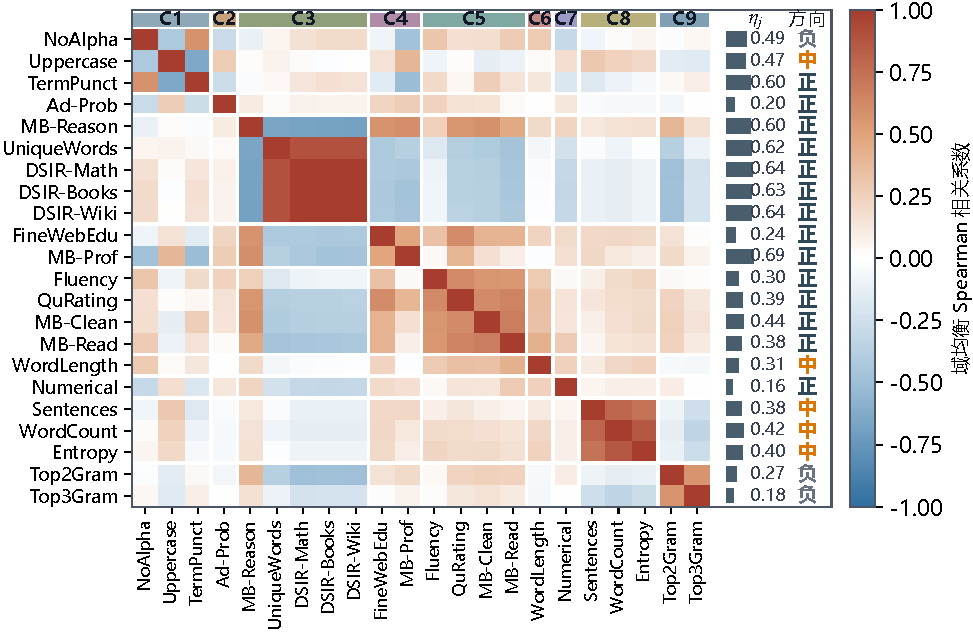
\includegraphics[width=0.78\textwidth]{figures/fig4_1_quality_structure.pdf}
    \caption{22 项质量信号的冗余结构与领域异质性}
    \label{fig:q1_quality_structure}
\end{figure}

\subsubsection{质量评价结果与一致性检验}
\label{subsubsec:q1_consistency}

领域级质量以域内 $Q_i^{(0)}$ 的均值表示，并在固定评价规则下采用分层 bootstrap 构造 95\% 置信区间。
表~\ref{tab:q1_q0_result} 给出七域点估计、分布中心和同源扩展检验，图~\ref{fig:q1_quality_evidence} 则展示领域排序及方向假设的主要证据。

\begin{table}[htbp]
    \TableSetup
    \caption{七域初始质量评价及同源扩展检验}
    \label{tab:q1_q0_result}
    \begin{tabular}{@{}C{2.30cm} C{1.25cm} C{1.85cm} C{2.65cm} C{1.85cm} C{1.60cm}@{}}
        \toprule
        领域 & $n$ & A1 均值 & 95\% CI & $\Delta Q$ & $W_1$ \\
        \midrule
        arxiv         & 1,419  & 0.7076 & [0.7055, 0.7098] & $-0.001740$ & 0.002437 \\
        commoncrawl   & 9,640  & 0.6056 & [0.6043, 0.6067] & -- & -- \\
        stackexchange & 10,000 & 0.6024 & [0.6011, 0.6038] & -- & -- \\
        wikipedia     & 10,000 & 0.5950 & [0.5934, 0.5968] & -- & -- \\
        c4            & 10,000 & 0.5548 & [0.5529, 0.5566] & -- & -- \\
        book          & 171    & 0.4994 & [0.4875, 0.5115] & -- & -- \\
        github        & 10,000 & 0.4786 & [0.4771, 0.4802] & $-0.000054$ & 0.000384 \\
        \midrule
        \multicolumn{2}{c}{总体} & \multicolumn{2}{c}{$Q_{\mathrm{micro}}=0.5707$} & \multicolumn{2}{c}{$Q_{\mathrm{macro}}=0.5776$} \\
        \bottomrule
    \end{tabular}
    \TableNote[0.94\textwidth]{注：A1 均值为初始质量 $Q^{(0)}$ 的域内均值，95\% CI 由分层 bootstrap 给出；$\Delta Q$ 为 A2/A3 全量均值减 A1 对应领域均值，$W_1$ 为 Wasserstein 距离。A2/A3 与 A1 同源，因此该结果用于检验抽样代表性。}
\end{table}

arxiv 的平均 $Q^{(0)}$ 最高，github 最低。github 的人工审阅相关仅为 0.071，明显低于其他领域，说明代码和技术文本与现有评价信号之间存在较强的领域失配；因此该排名仅表示统一评价口径下的相对位置，不作语料本身优劣的绝对判断。
A1 的微平均与宏平均接近，说明样本量不平衡未改变总体水平判断；book 样本量最小，其置信区间也最宽。
冻结 A1 的标量化规则、公共 ECDF、信息簇及簇内权重后应用于 A2/A3，arxiv 和 github 的均值差分别仅为 $-1.74\times10^{-3}$ 和 $-5.4\times10^{-5}$，对应的 Wasserstein 距离也很小，表明 A1 对两类同源扩展集合具有较好的代表性。

方向设定与聚合方式的消融结果见表~\ref{tab:q1_ablation}。最终“五中心”方案在保持七域排序稳定的同时，将 210 条分层人工复核与 $Q^{(0)}$ 的 Spearman 相关提高到 0.666；全部结构指标均按正向处理时，七域排序相关降至 0.429。
等权与 CRITIC 与本文方法的样本排序相关分别为 0.901 和 0.920，说明主要质量结构具有较高共识；全局 PCA 的一致性明显较低，说明直接以单一主成分压缩 22 项信号会损失部分质量语义。

\begin{table}[htbp]
    \TableSetup
    \caption{质量评价方案的消融与一致性检验}
    \label{tab:q1_ablation}
    \begin{tabular}{@{}C{1.60cm} C{3.20cm} C{1.70cm} C{1.70cm} C{3.10cm}@{}}
        \toprule
        检验类型 & 方案 & 七域排序 & 样本排序 & 人工审阅 \\
        \midrule
        \multirow{4}{*}{方向设定}
        & 旧八中心方案 & 1.000 & 0.880 & 0.616 [0.54, 0.68] \\
        & 最终五中心方案 & \textbf{1.000} & 1.000 & \textbf{0.666} [0.61, 0.72] \\
        & 中心指标减为四个 & 0.893 & 0.993 & 0.656 [0.60, 0.71] \\
        & 全部按正向处理 & 0.429 & 0.772 & 0.634 [0.56, 0.70] \\
        \addlinespace[2pt]
        \multirow{3}{*}{聚合基线}
        & 等权 & 0.929 & 0.901 & 0.619 [0.55, 0.69] \\
        & CRITIC & 0.929 & 0.920 & 0.625 [0.55, 0.69] \\
        & 全局 PCA & 0.750 & 0.622 & 0.449 [0.36, 0.53] \\
        \bottomrule
    \end{tabular}
    \TableNote{注：三列均为 Spearman 相关 $\rho_s$；人工审阅列为 210 条分层样本上的 95\% 分层 bootstrap 区间，样本按领域与质量层次分层抽取，排序相关均以最终五中心方案为基准。}
\end{table}

\begin{figure}[htbp]
    \centering
    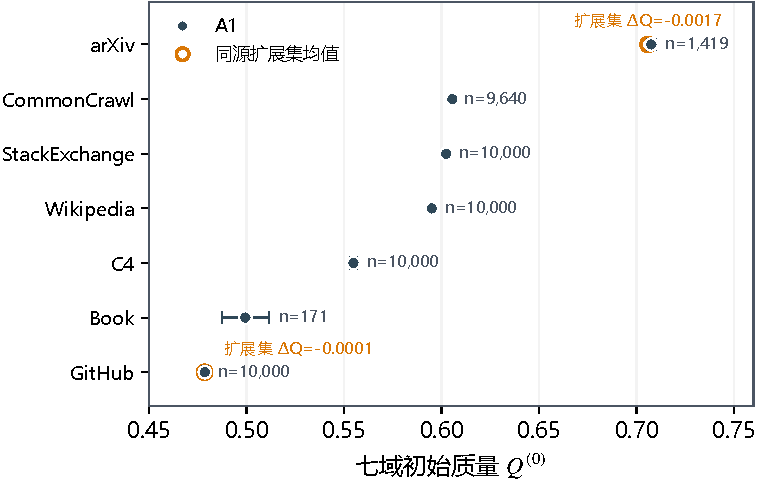
\includegraphics[width=0.64\textwidth]{figures/fig4_2_quality_evidence.pdf}
    \caption{七域质量评价结果与评价规则可信度}
    \label{fig:q1_quality_evidence}
\end{figure}

表~\ref{tab:q1_ablation} 的人工审阅列同时给出 210 条复核样本上的 95\% 分层 bootstrap 区间。最终五中心方案相对 CRITIC、等权和旧八中心方案的审阅相关差值分别为 0.041、0.047 和 0.050，区间分别为 $[0.009,0.073]$、$[0.013,0.080]$ 和 $[0.017,0.083]$，均不包含 0，说明方向审计与层次合成带来的提升不是抽样噪声，但幅度有限。
相对“中心指标减为四个”的差值为 0.010，区间 $[-0.003,0.022]$ 包含 0，二者在人工一致性上不可区分，保留中心五指标的意义在于不丢失结构语义；相对“全部按正向处理”的差值区间同样包含 0，该方案的决定性缺陷体现在七域排序相关由 1.000 降至 0.429。

由此得到的 $Q^{(0)}$ 保留了样本间的质量次序和域间差异，可作为下一节冲突校正的基准分数；其数值用于统一评价口径下的相对比较。

% -----------------------------------------------------
% 4.2 质量冲突消解
% -----------------------------------------------------
\subsection{质量冲突消解}
\label{subsec:q1_conflict}

$Q^{(0)}$ 的合成默认各项质量证据均可直接使用，但特殊文本可能使个别评价器偏离该领域的常见关系。
因此，本文把“正常的多维差异”与“异常的不一致”分开处理。只有当某项观测显著偏离同域相关信号所预测的正常水平时，才记为质量冲突；随后降低该项证据在综合评价中的权重。

\subsubsection{质量冲突的域感知识别}

以上一节的域均衡相关结构为基础，仅保留 $|\rho|\ge0.10$ 且在 300 次分层 bootstrap 中稳定率不低于 0.95 的指标关系，共得到 135 条稳定边。
对每项指标，用其稳定邻居和领域信息建立 Elastic Net 预测器，并按七域进行 5 折 cross-fitting，使每个样本的条件期望均由未包含该样本的训练折给出。
记交叉预测残差为 $e_{ij}=s_{ij}-\widehat s_{ij}^{(-i)}$，并在所属领域内按 MAD 标准化。若异常度进入对应“指标--领域”经验残差分布的上 2.5\% 尾部，则置 $I_{ij}=1$。样本级冲突度同时计入异常覆盖范围和异常强度，即
\begin{equation}
\begin{aligned}
r_{ij}&=\frac{|e_{ij}|}{1.4826\,\mathrm{MAD}_{d_i}(e_{\cdot j})+\varepsilon},\\
p_{ij}^{\mathrm{conf}}&=1-F_{j,d_i}^{R}(r_{ij}),\qquad
I_{ij}=\mathbf{1}\!\left\{p_{ij}^{\mathrm{conf}}<0.025\right\},\\
C_i&=\sqrt{\left(\frac{1}{22}\sum_j I_{ij}\right)
\left(\frac{\sum_j I_{ij}r_{ij}}{\sum_j I_{ij}+\varepsilon}\right)}.
\end{aligned}
\label{eq:q1_conflict}
\end{equation}
该定义以各指标在各领域中的正常波动为参照，因此不会把代码、公式密集文本等领域特征仅因数值差异而判为冲突。

\subsubsection{冲突证据的可靠性重加权}

冲突不直接从样本总分中扣除，而是作用于对应证据的可靠度。设 $\tau_{j,d_i}$ 为指标 $j$ 在领域 $d_i$ 的冲突阈值，定义
\begin{equation}
R_{ij}=\begin{cases}
1, & I_{ij}=0,\\
\exp\{-0.5(r_{ij}-\tau_{j,d_i})_+\}, & I_{ij}=1,
\end{cases}
\qquad
Q_i^*=\sum_{k=1}^{K}v_{ik}^*H_{ik},\quad
v_{ik}^*=\frac{\sum_{j\in G_k}a_{jk}R_{ij}}
{\sum_{\ell=1}^{K}\sum_{h\in G_\ell}a_{h\ell}R_{ih}}.
\label{eq:q1_qstar}
\end{equation}
各信息簇可靠度的均值记为 $U_i$。当不存在冲突时，$v_{ik}^*=1/K$，故 $Q_i^*=Q_i^{(0)}$；出现局部异常时，仅相应信息簇的权重发生变化。

\subsubsection{冲突消解效果及稳健性}

冲突校正后，$Q^*$ 与 $Q^{(0)}$ 的全样本 Spearman 为 0.9992，说明总体质量次序基本保持不变；但修正量明显向高冲突样本集中。
Top 10\%、Top 5\% 和 Top 1\% 冲突样本的 $|Q^*-Q^{(0)}|$ 中位数分别为 0.00435、0.00655 和 0.0118，且 Top 10\% 样本贡献了 64.8\% 的总绝对修正量。图~\ref{fig:q1_conflict_resolution} 中的分箱中位线进一步显示，冲突程度升高后修正幅度呈持续上升趋势。

\begin{figure}[htbp]
    \centering
    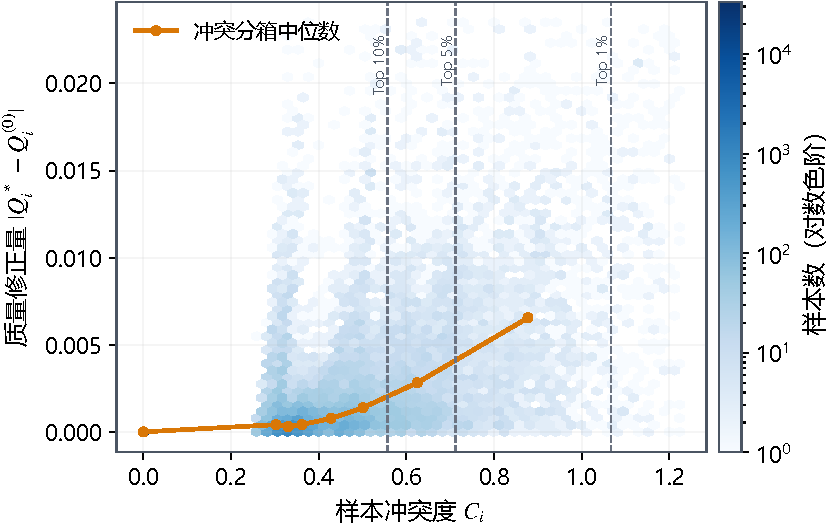
\includegraphics[width=0.66\textwidth]{figures/fig4_3_conflict_resolution.pdf}
    \caption{冲突修正的局部性与异常来源}
    \label{fig:q1_conflict_resolution}
\end{figure}

高严重度冲突主要集中在 Entropy、Sentences、Uppercase、WordCount 和 WordLength 等结构信号，表明异常主要来自文本结构偏离所属领域的常态。
最新结果中 GitHub 的平均冲突度最高（0.180），Book 最低（0.138）；这里的领域差异反映评价证据的一致性，而不用于比较领域质量高低。
将 A1 学得的关系结构、残差尺度和阈值冻结后应用于 A2/A3，严重冲突仍集中在同类结构信号。
作为对照，本文冲突度与“指标方差”和“最大两两差”的 Spearman 仅为 0.132 和 0.172；当显著性阈值在 0.01--0.10、可靠性衰减系数在 0.3--1.0 内变化时，$Q^*$ 排序与主方案的 Spearman 始终不低于 0.994。
因此，冲突校正主要影响高冲突尾部，并未改变质量评价的主体结构。第二小问最终输出 $(Q_i^*,U_i,C_i)$，分别记录修正后的质量、证据可信度和冲突程度。

% -----------------------------------------------------
% 4.3 领域配比—Loss关系
% -----------------------------------------------------
\subsection{领域配比--Loss关系}
\label{subsec:q1_mixture}

A4/A5 提供 512 组 1M 训练配方及其 13 域验证 Loss；A6/A7 为 1M 同尺度真实检验，A8/A9 和 A10/A11 分别提供 60M、1B 真实检验，A12--A15 为 10B、70B 外推表。
17 个训练比例满足 $p_i\ge0$、$\sum_i p_i=1$，而 13 个验证域的 Loss 基准不同，因此建模时需同时处理单纯形约束、多输出响应和跨尺度迁移。

\subsubsection{配比数据标准化及质量先验检验}

不同验证域的 Loss 先在 A5 内按验证域进行中位数--MAD 标准化，再定义总体配比表现，即
\begin{equation}
z_{mk}=\frac{L_{mk}-\operatorname{median}(L_{\cdot k})}
{1.4826\,\operatorname{MAD}(L_{\cdot k})},\qquad
\phi(\mathbf p)=-\frac{1}{13}\sum_{k=1}^{13}\widehat z_k(\mathbf p).
\label{eq:q1_phi}
\end{equation}
$\phi(\mathbf p)$ 越大，表示该配方在 13 个验证域上的总体表现越优。

第二小问得到的七域 $Q^*$ 经 A16 映射到 17 个训练域。由于 $\sum_i p_iQ_i$ 是 $\mathbf p$ 的确定函数，直接作为额外线性项会与配比变量共线。
因此以指数倾斜 $\widetilde p_i(\gamma)\propto p_i\exp[\gamma(Q_i-\bar Q)]$ 检验质量先验。交叉验证的最优值为 $\gamma=0$，且 $\gamma>0$ 时误差略有增加，说明 A4/A5 无法把“领域身份”与“领域质量”的独立作用分开识别。
本小问据此不引入质量先验，质量的独立边际效应在问题二 B6--B8 的独立质量变化中进一步估计。

\subsubsection{配比--Loss 响应的预测与解释模型}

为显式刻画领域及领域组合的作用，对第 $k$ 个验证域建立二阶 Scheff\'e 混合响应
\begin{equation}
\widehat z_k(\mathbf p)=\sum_{i=1}^{17}\beta_{ik}p_i+
\sum_{1\le i<j\le17}\gamma_{ijk}p_ip_j,
\qquad k=1,\ldots,13.
\label{eq:q1_scheffe}
\end{equation}
17 个主效应和 136 个交互项在 13 个任务上联合拟合，以组稀疏约束筛选跨任务稳定结构，并用 Ridge 项稳定相关系数；一阶 Scheff\'e 和 ILR--Ridge 作为对照。
1M 真实检验结果见表~\ref{tab:q1_mixture_model}。

\begin{table}[htbp]
    \TableSetup
    \caption{1M 真实检验集上的配比响应模型比较}
    \label{tab:q1_mixture_model}
    \begin{tabular}{@{}C{3.40cm} C{2.20cm} C{2.00cm} C{1.60cm} C{2.80cm}@{}}
        \toprule
        模型 & 平均 RMSE & 平均 $R^2$ & MAE & 用途 \\
        \midrule
        一阶 Scheff\'e & 0.522 & 0.619 & 0.435 & 线性混合基准 \\
        多任务稀疏 Scheff\'e & 0.444 & 0.710 & 0.361 & 机制解释 \\
        ILR--Ridge & \textbf{0.420} & \textbf{0.765} & \textbf{0.337} & 数值预测 \\
        \bottomrule
    \end{tabular}
    \TableNote{注：RMSE、$R^2$、MAE 均为 13 个验证任务的平均值；总体宏观配比指标 $G$ 在 1M 检验集上的 $R^2$ 为 0.391。}
\end{table}

ILR--Ridge 的点估计最优；重复 5 折交叉验证下，其相对多任务 Scheff\'e 的 $R^2$ 差值均值为 0.038，95\% CI 为 $[-0.012,0.081]$，区间包含 0。
因此后续数值预测采用 ILR--Ridge，领域替换和交互机制采用多任务稀疏 Scheff\'e 解释，两类模型分别承担预测和机制分析任务。

\subsubsection{领域份额替换及互补结构}

在单纯形约束下，“增加领域 $i$”必然伴随其他领域份额减少，因此主效应系数不能直接解释为独立边际收益。
在参考配比 $\mathbf p$ 附近，定义从领域 $j$ 向领域 $i$ 转移份额的边际效应和两领域的总体互补指数，即
\begin{equation}
S_{i\leftarrow j}(\mathbf p)=\frac{1}{13}\sum_{k=1}^{13}
\left(\frac{\partial\widehat z_k}{\partial p_i}-\frac{\partial\widehat z_k}{\partial p_j}\right),\qquad
C_{ij}^{\mathrm{mix}}=-\frac{1}{13}\sum_{k=1}^{13}\gamma_{ijk}.
\label{eq:q1_sub_comp}
\end{equation}
$S_{i\leftarrow j}<0$ 表示在当前配比附近将份额从 $j$ 转移到 $i$ 有助于降低总体 Loss；$C_{ij}^{\mathrm{mix}}>0$ 表示两域共同出现时的 Loss 低于线性混合预期。
前者描述份额替换，后者描述非加性交互。

为控制稀疏配方造成的大系数伪影，正文只解释同时满足三项条件的关系，即两域训练覆盖充分、bootstrap 符号稳定率不低于 0.95、效应量位于训练支持范围。
约 52\% 的替换关系和 46\% 的互补关系通过该门槛。通过门槛的关系中，DM-Math $\rightarrow$ HackerNews 的替换效应为 $-2.68$，显示稳定的 Loss 改善信号；arXiv--GitHub 则表现出稳定互补。
相反，\texttt{enron\_emails} 的平均份额仅 0.0022、最大份额 0.026、非零占比 0.31，其大幅替换效应超出充分支持范围，因此不进入机制结论。
图~\ref{fig:q1_mixture_mechanism} 将替换矩阵和通过资格门槛的互补/冗余关系合并展示，灰色斜线区域表示证据不足。

\begin{figure}[htbp]
    \centering
    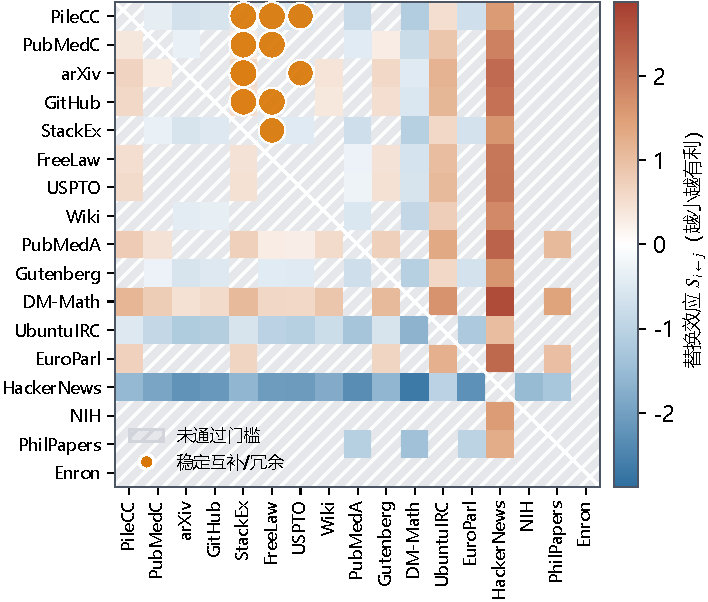
\includegraphics[width=0.68\textwidth]{figures/fig4_4_mixture_mechanism.pdf}
    \caption{领域配比的替换机制与互补结构}
    \label{fig:q1_mixture_mechanism}
\end{figure}

\subsubsection{配比规律的跨尺度迁移边界}

同尺度预测精度不能直接代表跨规模可迁移性，因此分别考察配比空间外推和模型规模迁移。
在配比空间内，以 Hellinger 距离衡量测试配方到最近训练配方的距离。1M 检验集最近邻距离的中位数为 0.299，90\% 分位数为 0.375，且预测误差随距离增大而整体上升，说明模型的机制解释应限制在训练配方支持区域附近。

模型规模迁移通过不同尺度下的配方排序一致性衡量。表~\ref{tab:q1_cross_scale} 和图~\ref{fig:q1_transfer_boundary} 显示，60M 和 1B 的 Spearman 相关分别为 0.810 和 0.608，均保持为正，但随规模扩大明显减弱；10B、70B 的 Loss 为较小规模幂律外推结果，其排序相关和预测--观测斜率均转为负值。
因此，现有数据支持真实 1M--1B 范围内的有限迁移，不支持将小模型上的配比规律视为尺度不变关系。

\begin{table}[htbp]
    \TableSetup
    \caption{领域配比效应的跨尺度一致性}
    \label{tab:q1_cross_scale}
    \begin{tabular}{@{}C{1.90cm} C{1.90cm} C{1.40cm} C{2.40cm} C{2.00cm} C{2.00cm}@{}}
        \toprule
        模型规模 & 数据性质 & 样本数 & 排序相关 $\rho_s$ & 两两一致率 & 回归斜率 \\
        \midrule
        60M & 真实检验 & 256 & 0.810 & 0.805 & 0.912 \\
        1B  & 真实检验 & 64  & 0.608 & 0.711 & 0.348 \\
        \addlinespace[2pt]
        10B & 外推 Loss & 63 & $-0.584$ & 0.293 & $-0.339$ \\
        70B & 外推 Loss & 63 & $-0.617$ & 0.279 & $-0.370$ \\
        \bottomrule
    \end{tabular}
    \TableNote[0.94\textwidth]{注：排序相关为各尺度配方排序与 1M 预测排序的 Spearman 相关，两两一致率为配方两两比较方向一致的比例，回归斜率为预测--观测回归的斜率；10B/70B 的 Loss 来自小规模实验的幂律外推，仅用于识别尺度失效边界，不作为真实大模型训练验证。}
\end{table}

\begin{figure}[htbp]
    \centering
    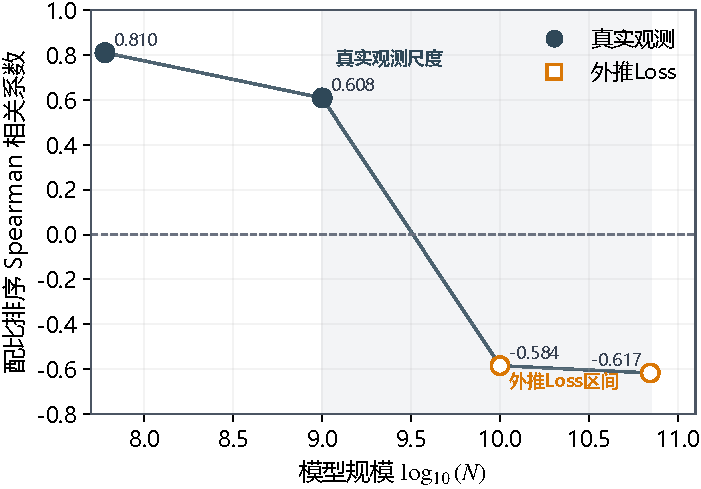
\includegraphics[width=0.64\textwidth]{figures/fig4_5_transfer_boundary.pdf}
    \caption{配比模型的预测有效域与跨尺度迁移边界}
    \label{fig:q1_transfer_boundary}
\end{figure}

问题一最终得到三类后续输入，即冲突修正质量 $Q^*$、映射到 17 个训练域的质量描述 $Q^{(17)}$ 以及总体配比效应 $\phi(\mathbf p)$。
替换效应 $S_{i\leftarrow j}$ 和互补指数 $C_{ij}^{\mathrm{mix}}$ 用于解释领域结构，$U$ 与 $C$ 用于记录质量评价中的不确定性。
问题二将在此基础上融合附件 B，建立含参数规模、数据量、质量和领域结构的广义标度关系。

% =====================================================
% 五、问题二
% =====================================================
\section{问题二：广义标度律及质量--规模替代}
% TODO

% =====================================================
% 六、问题三
% =====================================================
\section{问题三：算力约束下的联合资源配置}
% TODO

% =====================================================
% 七、问题四
% =====================================================
\section{问题四：技术演进分解及能力前沿预测}
% TODO

% =====================================================
% 八、结论、局限与推广
% =====================================================
\section{结论、局限与推广}
% TODO

\clearpage

\bibliographystyle{gmcm}
\bibliography{reference}

\clearpage

\section*{AI 工具使用说明}
本文使用 AI 工具辅助数据字段理解、代码调试、图表绘制、文字润色，以及对 210 条分层抽样文本进行初步阅读。
上述 AI 输出均由作者逐项复核并独立确认，论文中采用的原文一致性结论以作者复核结果为准。
核心模型、公式推导、参数选择、结果解释与结论由作者完成。

\clearpage

\begin{appendices}
    \section{完整数据审计表}
    % TODO

    \section{关键参数与敏感性结果}
    % TODO

    \section{程序代码}
    % TODO
\end{appendices}

\end{document}
